
\chapter{Planning}
\label{chap:plan}

In questo capito si andranno ad analizzare i compiti della seconda fase all'interno del ciclo della
\hyperref[sec:pipeline]{pipeline dei veicoli autonomi}, ovvero il planning. In questa fase viene inserito
l'argomento di studio di questa tesi: \textit{l'ottimizzazione della traiettoria globale}.
Il planning, come suggerisce il nome, ha il compito di pianificare le mosse successive del robot affinché
possa spostarsi in modo ottimale evitando eventuali ostacoli.

\bigskip
\noindent Gli algoritmi si differenziano per tecniche e obiettivi, in particolare si distinguono tre
macro-categorie che rispondono a domande diverse:
\begin{itemize}
	\item \textbf{Mission/Global Planner}: \textit{Qual è l'obiettivo generale del veicolo?} Per esempio trovare
	il percorso più breve, o quello più corto; 
	\item \textbf{Behavioural Planner}: \textit{Come dovrebbe comportarsi il veicolo in diverse situazioni?} Per
	esempio, in una gara con più concorrenti, quando superare un avversario, come e dove;
	\item \textbf{Local Planner}: \textit{Quali sono le traiettorie possibili dalla posizione attuale al goal?}
	Per esempio trovare la miglior traiettoria tale che rientri nella possibilità fisica del veicolo.
\end{itemize}
L'oggetto di questa tesi, l'ottimizzazione della traiettoria di corsa, rientra nella prima categoria.

\paragraph{\textit{Workspace} vs \textit{Configuration Space}} \ \\
Si distinguono due rappresentazioni degli ostacoli e dell'ambiente: il workspace rappresenta tutte le
\textit{azioni possibili} a un robot, si pensi al volume occupato da tutti i possibili movimenti di un
braccio meccanico, mentre il configuration space, detto anche C-space, rappresenta tutte le possibili
configurazioni di una data \textit{definizione di stato}. In questo contesto, all'atto pratico, ciò si
traduce che nel secondo, la rappresentazione dell'ambiente e degli ostacoli tiene già conto della
\textit{dimensione} del robot e quindi può essere considerato come un singolo punto, mentre ciò non
accade nel primo. La figura \ref{fig:work-vs-conf-space} ne mostra un esempio.
\begin{figure}[H]
	\begin{center}
		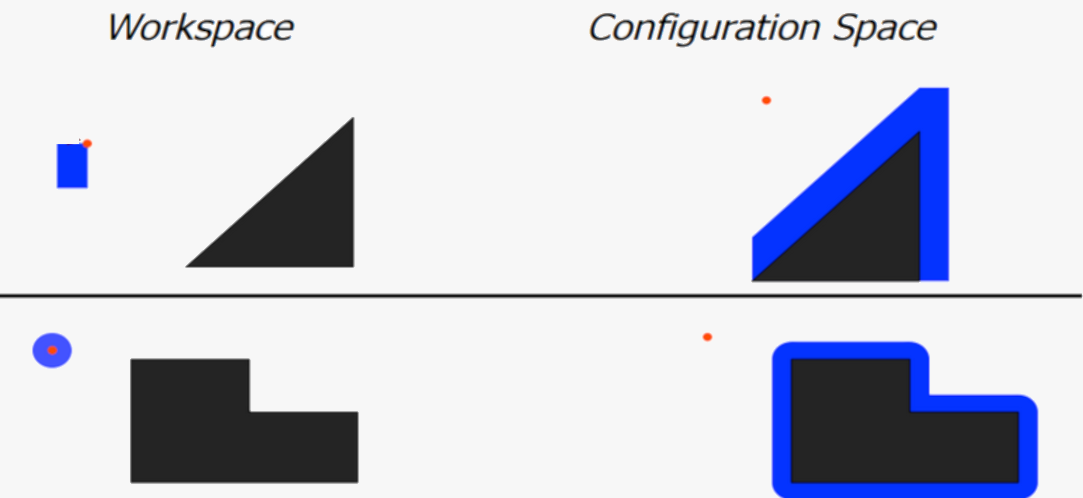
\includegraphics[width=0.95\textwidth]{work-vs-conf-space.png}
	\end{center}
	\caption{Differenze tra Workspace e C-Space~\cite{lection11}; in nero la dimensione degli ostacoli
	reali, in rosso il punto di controllo del robot, in blu, nel caso workspace, lo spazio occupato dal
	robot, mentre per C-Space, lo spazio che occuperebbe vicino agli ostacoli}
	\label{fig:work-vs-conf-space}
\end{figure}
Nel contesto delle corse si preferisce l'uso del C-space per via della usa \textit{espressività} nella
descrizione dello stato, che può non solo descrivere un piano o uno spazio tridimensionale, ma è
possibile esprimere ulteriori variabili come la velocità e l'orientamento: è così possibile esprimere
\textit{ulteriori vincoli}.

\bigskip
\noindent Di seguito si analizzano le tre macro-categorie sopra citate.

\section{Local Planner}
L'obiettivo principale del local planner è quello pianificare i movimenti del robot fino ad un dato
orizzonte finito evitando collisioni con l'ambiente ed eventuali avversari. Gli algoritmi si
differenziano per tre categorie principali di risoluzione:
\begin{enumerate}
	\item Applicando \textit{modifiche} la raceline globale; 
	\item \textit{Generando diverse traiettorie} vincolate alla dinamica del robot e scegliendo quella migliore;
	\item \textit{Campionando} lo spazio libero e trovando un percorso attorno agli ostacoli.
\end{enumerate}
Nella prima categoria rientrano, generalmente, algoritmi che si basano su MPC che, sebbene sia un
algoritmo di controllo ottimale, può essere adattato e utilizzato per ricercare il percorso ottimo per
evitare un ostacolo o per migliorare la traiettoria della raceline globale di riferimento in base alla
posizione attuale del veicolo.

Nella seconda categoria ricadono algoritmi che calcolano, fino a un dato orizzonte temporale, lo stato
successivo del veicolo per diversi input di accelerazione e angolo delle ruote; questa operazione produce
diverse traiettorie, dinamicamente praticabili per il robot, da cui si sceglie la migliore secondo una
funzione di costo. Altri algoritmi, come State Lattice, generano punti equidistanti nell'ambiente tra di
loro connessi da delle \hyperref[par:spline-def]{spline} che seguono la dinamica del veicolo, poi viene
ricercato il percorso migliore. Un esempio grafico è mostrato in figura \ref{fig:state-lattice}.

La terza categoria, data una occupancy grid e un punto di goal, algoritmi come PRM (Probabilistic Road
Map) e derivati come RRT (Rapidly-Exploring Random Tree) campionano lo spazio libero e generano un grafo
che connette i punti campionati per poi cercare il percorso che avvicina il robot al goal. RRT è stato un
caso di studio durante questa tesi durante un laboratorio del Modulo D. Un esempio di RRT si può trovare
alla figura \ref{fig:rviz-example}. Altre soluzioni usano i classici algoritmi di ricerca su grafo, come
A* e Dijkstra, sulla stessa occupancy grid; il grafo costruito a partire da essa esprime sui nodi le posizioni
nell'ambiente e gli archi i possibili input da quelle posizioni. Queste ultime sono soluzioni che
lavorano nel discreto, molto semplici da implementare ma che non hanno la stessa espressività dei metodi
continui e che non hanno la possibilità di descrivere la dinamica del robot.

\begin{figure}[H]
	\begin{center}
		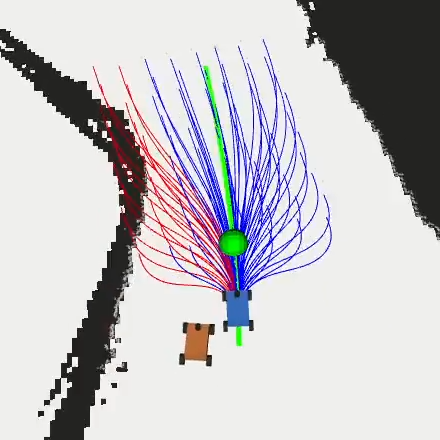
\includegraphics[height=0.3\textheight]{state-lattice.png}
	\end{center}
	\caption{Esempio grafico dell'algoritmo State Lattice \cite{state-lattice}}
	\label{fig:state-lattice}
\end{figure}

\section{Behavioural Planner}
Il focus di questo planner è generalmente selezionare un peso appropriato a diversi obiettivi o combinare
il risultato del local planner con metodi della teoria del gioco così da pianificare delle mosse atte a
impedire il progresso degli avversari.

Nel primo caso, gli obiettivi rappresentano valori come il progresso sul circuito, la vicinanza con gli
ostacoli e contendenti, la deviazione dal percorso ottimale, la velocità massima; il costo totale di una
traiettoria viene quindi calcolato combinando secondo vari pesi gli obiettivi presi in considerazione,
viene quindi scelto la traiettoria col costo minore.

Nel secondo caso vengono sfruttate metodologie della teoria dei giochi per trovare l'azione migliore in
un ambiente con due o più giocatori. Il problema viene trasformato in gioco competitivo asincrono dove un
singolo giocatore può "muoversi" per volta. Questi approcci spesso includono nel calcolo della soluzione il
concetto di \textit{regret} per trovare la migliore risposta per vincere la gara.

\section{Global Planner}
Come citato più volte precedentemente, questa tipologia di planner è stato oggetto di studio di questa
tesi e quindi ha dedicato un capitolo, il numero \ref{chap:opt} (pag. \pageref{chap:opt}).

Il global planner ha una visione d'insieme del circuito ed è agnostico alla singola gara, perciò i suoi
obiettivi sono legati a proprietà della traiettoria (globale) da seguire; generalmente l'obiettivo
principale è eseguire il tracciato in meno tempo possibile, ma esistono altre possibilità come il minor
consumo d'energia e traiettorie con particolari proprietà geometriche, come la minor curvatura.

